\documentclass{article}

\usepackage{lmodern}
\usepackage{hyperref}
\usepackage{amsmath}
\usepackage{amssymb}
\usepackage[T1]{fontenc}
\usepackage{fancyhdr}
\usepackage{color,graphicx}
\pagestyle{fancy}
\lhead{Anirudhan J Rajagopalan --- ajr619}
\lhead{Michele Ceru --- mc3784}

\begin{document}

\title{Deep Learning --- Homework 1}
\date{February 11, 2016}
\author{Anirudhan J Rajagopalan, Michele Ceru\\ ajr619, mc3784}

\maketitle

\newpage

\section[Expression for energy]{Backpropogation}
\begin{enumerate}
\item Using the chain rule:
$$
\frac{\partial E}{\partial x_{\text{in}}} = \frac{\partial E}{\partial x_{\text{out}}}\frac{\partial x_{\text{out}}}{\partial x_{\text{in}}}
$$  
Using the expression of $x_{\text{out}}$ given in the question we have:
$$
\frac{\partial x_{\text{out}}}{\partial x_{\text{in}}} = \frac{\partial }{\partial x_{\text{in}}} \big(\frac{1}{1+e^{-x_{\text{in}}}}\big) = \frac{e^{-x_{\text{in}}} }{(1+e^{-x_{\text{in}}})^2}
$$
Summing and subtracting $1$ in the numerator:
$$
\frac{\partial x_{\text{out}}}{\partial x_{\text{in}}}  = \frac{1+e^{-x_{\text{in}}} -1}{(1+e^{-x_{\text{in}}})^2}=\frac{1}{1-e^{-x_{\text{in}}}}\Big[  1-\frac{1}{1-e^{-x_{\text{in}}}}\Big]
$$
And using the expression of $x_{\text{out}}$ given in the question:
$$
\frac{\partial E}{\partial x_{\text{in}}} =\frac{\partial E}{\partial x_{\text{out}}}x_{\text{out}}[1-x_{\text{out}}]
$$

\item Using the expression of $x_{\text{out}}$ given in the question:
$$
\frac{\partial (x_{\text{out}})_i}{\partial (x_{\text{in}})_j} = \frac{\partial }{\partial (x_{\text{in}})_j} \Big(  
\frac{e^{-\beta (x_{\text{in}})_i}}{\sum_k e^{-\beta (x_{\text{in}})_k}}
\Big)
$$
In the case $i=j$:
$$
\frac{\partial (x_{\text{out}})_i}{\partial (x_{\text{in}})_i} =    
\frac{-\beta e^{-\beta (x_{\text{in}})_i} (\sum_k e^{-\beta (x_{\text{in}})_k} )- e^{-\beta (x_{\text{in}})_i} (-\beta e^{-\beta (x_{\text{in}})_i}   )
}
{\sum_k e^{-\beta (x_{\text{in}})_k}}=
$$

$$
=-\frac{\beta e^{-\beta (x_{\text{in}})_i}}{\sum_k e^{-\beta (x_{\text{in}})_k} } \Big[  1-\frac{\beta e^{-\beta (x_{\text{in}})_i}}{\sum_k e^{-\beta (x_{\text{in}})_k} }\Big]
$$and substituting the expression of $x_{\text{out}}$:
$$
\frac{\partial (x_{\text{out}})_i}{\partial (x_{\text{in}})_i} =\beta  (x_{\text{out}})_i [1- (x_{\text{out}})_i]
$$
In the case $i\neq j$:
$$
\frac{\partial (x_{\text{out}})_i}{\partial (x_{\text{in}})_j} =    
-\beta e^{-\beta (x_{\text{in}})_j} (\sum_k e^{-\beta (x_{\text{in}})_k} )^{-2} e^{-\beta (x_{\text{in}})_i} =
$$ 
$$
=\beta \frac{e^{-\beta (x_{\text{in}})_j}}{\sum_k e^{-\beta (x_{\text{in}})_k} }
\frac{e^{-\beta (x_{\text{in}})_i}}{\sum_k e^{-\beta (x_{\text{in}})_k} } =\beta (x_{\text{out}})_j(x_{\text{out}})_i 
$$
Writing the solution all together:
\begin{equation*}
      \frac{\partial (x_{\text{out}})_i}{\partial (x_{\text{in}})_j} = \begin{cases}
                       \beta  (x_{\text{out}})_i [1- (x_{\text{out}})_i]   \text{\,	if  $i= j$}\\
                        \beta (x_{\text{out}})_j(x_{\text{out}})_i   \text{\,	if  $i\neq j$}
                    \end{cases}
\end{equation*}

\end{enumerate}

\section[Kaggle contest]{Torch (MNIST handwriting recognition)}

\subsubsection{Model file}
  The model file can be found at \href{http://cs.nyu.edu/~ajr619/model.net}{http://cs.nyu.edu/~ajr619/model.net}
\subsubsection{Github repo}
  The repository for the changes and result.lua is at \\
  \href{https://github.com/rajegannathan/Deep-Learning/tree/master/hw1}{https://github.com/rajegannathan/Deep-Learning/tree/master/hw1}
\subsubsection{Best performing model}
  We got a best test set performance of 99.57\% for a slightly modified convolutional net wherein we rotate the image by angles produced by normal distribution with 0 mean and 0.2 deviation.  The randomly generated values are taken as the radians by which the image should be rotated.
\subsubsection{Experiments}
\subsubsection{Figures}
\begin{figure}[ht!]
  \centering
  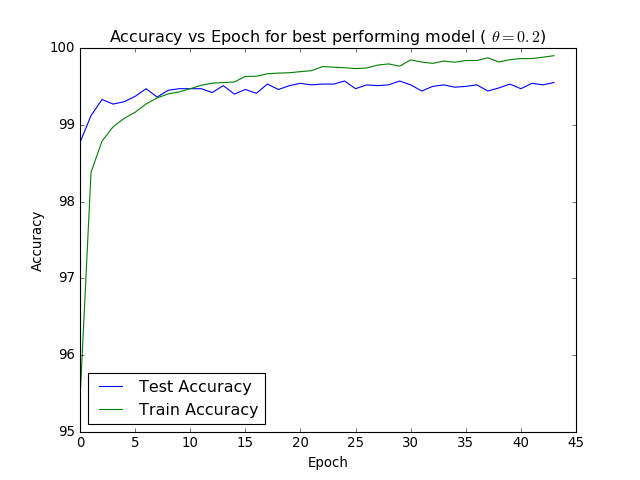
\includegraphics[width=1\textwidth]{bestPerformance}
  \caption{Sample Data format.  The columns correspond to id,  Fp1, Fp2, F7, F3, Fz, F4, F8, FC5, FC1, FC2, FC6, T7, C3, Cz, C4, T8, TP9, CP5, CP1, CP2, CP6, TP10, P7, P3, Pz, P4, P8, PO9, O1, Oz, O2, PO10.\label{fig:Sample_data}}
\end{figure}
\begin{figure}[ht!]
  \centering
  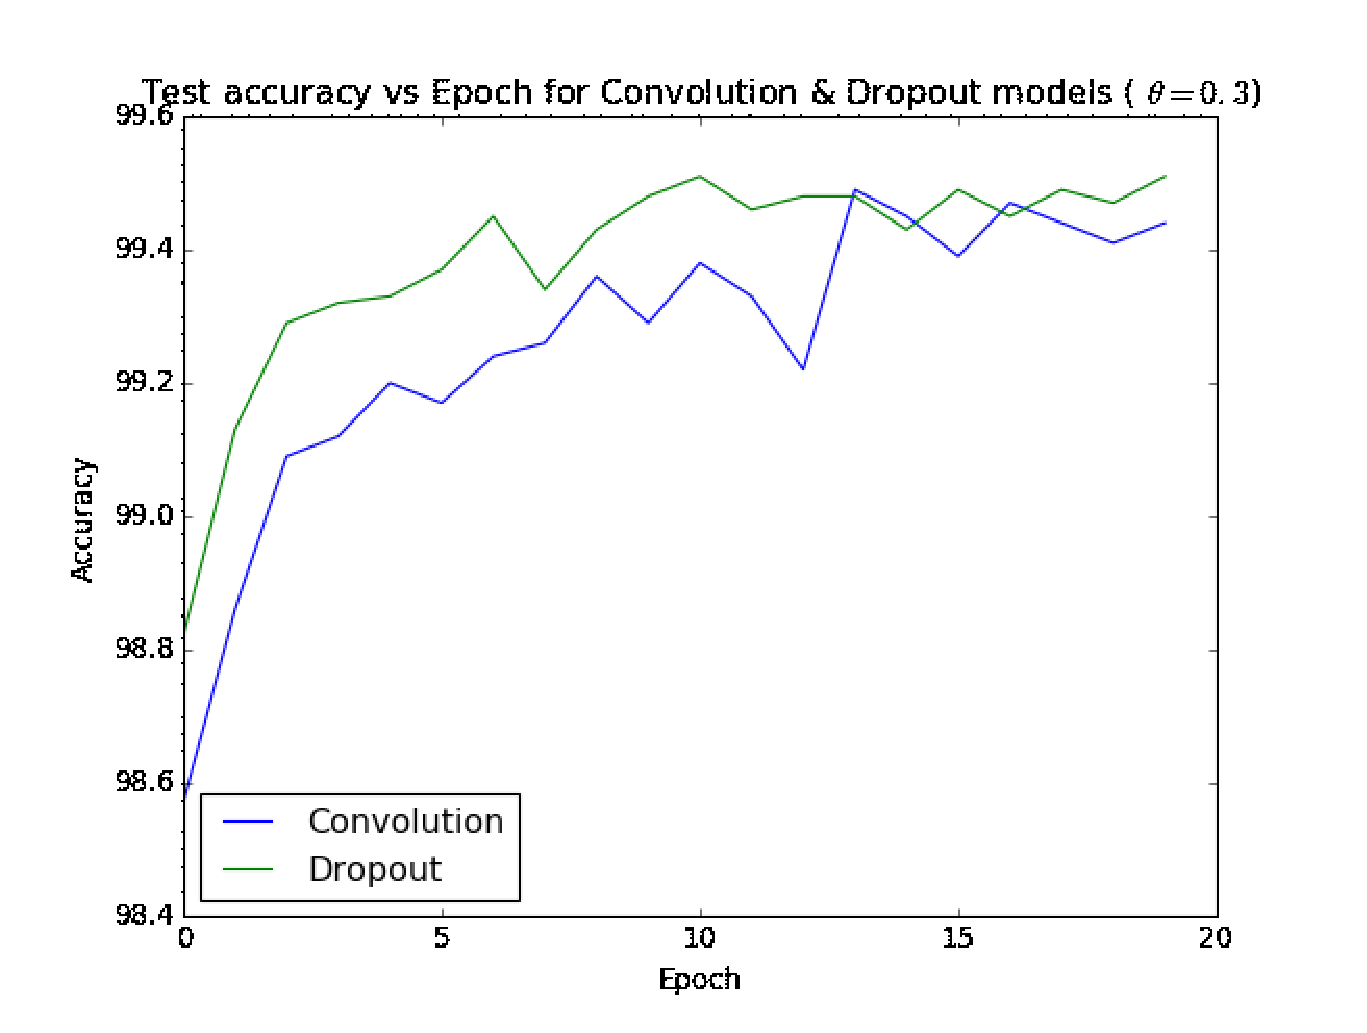
\includegraphics[width=1\textwidth]{convolution_dropout}
  \caption{Sample Data format.  The columns correspond to id,  Fp1, Fp2, F7, F3, Fz, F4, F8, FC5, FC1, FC2, FC6, T7, C3, Cz, C4, T8, TP9, CP5, CP1, CP2, CP6, TP10, P7, P3, Pz, P4, P8, PO9, O1, Oz, O2, PO10.\label{fig:Sample_data}}
\end{figure}
\end{document}
